\documentclass{acm_proc_article-sp}

\usepackage[utf8]{inputenc}
\usepackage[T1]{fontenc}
\usepackage[activate=compatibility]{microtype}

% autoref command
\usepackage[pdftex,urlcolor=black,colorlinks=true,linkcolor=black,citecolor=black]{hyperref}
\def\sectionautorefname{Section}
\def\subsectionautorefname{Subsection}
\def\subfloatautorefname{Subfigure}

\usepackage[lofdepth,lotdepth]{subfig}
\usepackage{enumitem}
\usepackage{textcomp}
\usepackage{mathtools}
\usepackage{url}

% give emph a normal fontsize
\let\oldemph\emph
\renewcommand{\emph}[1]{\oldemph{\fontsize{9}{9}\selectfont #1}}

% more readable footnote layout
\renewcommand{\footnotesize}{\fontsize{8pt}{10pt}}
\setlength{\footnotesep}{.5cm}

% todo macro
\usepackage{color}
\newcommand{\todo}[1]{\noindent\textcolor{red}{{\bf \{TODO}: #1{\bf \}}}}

% listings and Verbatim environment
\usepackage{fancyvrb}
\usepackage{relsize}
\usepackage{listings}
\usepackage{verbatim}
\newcommand{\defaultlistingsize}{\fontsize{8pt}{9.5pt}}
\newcommand{\inlinelistingsize}{\fontsize{8pt}{11pt}}
\newcommand{\smalllistingsize}{\fontsize{7.5pt}{9.5pt}}
\newcommand{\listingsize}{\defaultlistingsize}
\RecustomVerbatimCommand{\Verb}{Verb}{fontsize=\inlinelistingsize}
\RecustomVerbatimEnvironment{Verbatim}{Verbatim}{fontsize=\defaultlistingsize}
\lstset{frame=lines,captionpos=b,numberbychapter=false,escapechar=§,
        aboveskip=0.5em,belowskip=0em,abovecaptionskip=0em,belowcaptionskip=0em,
framexbottommargin=-1em,
        basicstyle=\ttfamily\listingsize\selectfont}

\usepackage{color}
\definecolor{lightgray}{rgb}{.9,.9,.9}
\definecolor{darkgray}{rgb}{.4,.4,.4}
\definecolor{purple}{rgb}{0.65, 0.12, 0.82}

\lstdefinelanguage{JavaScript}{
  keywords={typeof, new, true, false, catch, function, return, null, catch, switch, var, if, in, while, do, else, case, break},
  keywordstyle=\color{blue}\bfseries,
  ndkeywords={class, export, boolean, throw, implements, import, this},
  ndkeywordstyle=\color{darkgray}\bfseries,
  identifierstyle=\color{red},
  sensitive=false,
  showstringspaces=false,
  comment=[l]{//},
  morecomment=[s]{/*}{*/},
  commentstyle=\color{purple}\ttfamily,
  stringstyle=\color{gray}\ttfamily,
  morestring=[b]',
  morestring=[b]"
}

% use Courier from this point onward, except for URLs
\let\oldttdefault\ttdefault
\renewcommand{\ttdefault}{pcr}
\let\oldurl\url
\renewcommand{\UrlFont}{\fontfamily{\oldttdefault}\selectfont}

% linewrap symbol
\definecolor{grey}{RGB}{130,130,130}
\newcommand{\linewrap}{\raisebox{-.6ex}{\textcolor{grey}{$\hookleftarrow$}}}

% for 1st, 2nd, etc. superscripting
\newcommand{\ts}{\textsuperscript}

% more pleasing quote environment
\usepackage{tikz}
\newcommand*{\openquote}{\tikz[remember picture,overlay,xshift=-7pt,yshift=1pt]
     \node (OQ) {\fontfamily{fxl}\fontsize{16}{16}\selectfont``};\kern0pt}
\newcommand*{\closequote}{\tikz[remember picture,overlay,xshift=2pt,yshift=-4.5pt]
     \node (CQ) {\fontfamily{fxl}\fontsize{16}{16}\selectfont''};}
\renewenvironment{quote}%
{\setlength{\parindent}{1cm}\par\openquote}
{\closequote\vspace{-4.5pt}
}

\begin{document}

\title{NiteOutMag\hspace{-1.5pt}\raisebox{6pt}{$^\textbf{\sffamily TM}$}---At Least the Web\\ Remembers What Happened Last Night}

\numberofauthors{2}
\author{
% Tom, Ruben, Raphaël, Giuseppe, José
}
\maketitle

\begin{abstract}
The chorus of the popular song \emph{Tik Tok} by the artist \emph{Ke\$ha} goes
\emph{``Don't stop, make it pop. DJ, blow my speakers up. Tonight, I'mma fight.
'Til we see the sunlight. Tik tok on the clock. But the party don't stop, no.''}
We all know, however, that each party comes to an end eventually.
With NiteOutMag\texttrademark, we present a~Chrome Web application
that can help people recover what (the hell) happened last night.
Among the younger generation, nightlife activities---just about like any other
activity---together with related multimedia data get shared online on social networks.
The problem is that for one and the same event, the event-related user-generated data
may be shared on a~plethora of social networks.
Therefore, for this challenge, we introduce an application
that leverages event data from several event databases,
social data from multiple social networks, and media data from some media platforms.
The collected data for events around a~given area is then compiled
in an event-centric magazine-like way, where each page represents one event.
Just like the nightlives of people happen \emph{ad hoc} from one party to the other,
the NiteOutMag\texttrademark~application as well
gathers all its data on-the-fly, without the burden of pre-compiled data directories.
The application is available online\footnote{\todo{Add demo link}}.
A~screencast showcasing the application is also available\footnote{\todo{Add screencast link}}.
\end{abstract}

%\category{H.3.4}{Information Systems}{Information Storage and Retrieval}[World Wide Web]
%\category{H.3.5}{Online Information Services}{Web-based services}

%\keywords{}


\section{Introduction}
In March 2012, the at the time 901 million monthly active users
of the social networking site (SNS) Facebook
have uploaded more than 300 million photos on average per day~\cite{Facebook2012}.
Many of those photos are event-related, \emph{e.g.},
illustrate events like music concerts that a~social network user has attended.
Facebook, however, albeit the biggest, is only one among a~plethora of social networks
that event attendants may have shared their event-related content on.
In the next subsection, we thus list the SNSs considered for
NiteOutMag\texttrademark.

\subsection{Social Networks} \label{sec:social-networks}
A~social network is an online service or media platform that focuses on building
and reflecting social relationships among people sharing interests and/or activities.
In this paper, we consider eleven different social networks
that represent all together most of the Western world's market share.
In detail, the considered social networks are
\mbox{Google+} (\url{google.com/+}),
Myspace (\url{myspace.com}),
Facebook (\url{facebook.com}),
Twitter ({twitter.com}),
Instagram (\url{instagram.com}),
Flickr (\url{flickr.com}),
YouTube (\url{youtube.com}),
yfrog (\url{yfrog.com}),
MobyPicture (\url{mobypicture.com}),
Twitpic (\url{twitpic.com}), and
\mbox{img.ly} (\url{img.ly}).

The actual detection of events based on information from SNSs
is out of bounds for this paper.
We point the reader to, \emph{e.g.},~\cite{Petkos2012} by Petkos \emph{et al.},
which is a~typical example of event detection based on multimodal clustering.
For our purposes, event databases as listed below are adequate.

\subsection{Event Databases}
An event database is an online service that holds metadata
for a~categorized set of events that can be queried programmatically.
We consider four event databases, namely
Eventful (\url{eventful.com}),
Foursquare (\url{foursquare.com}),
Upcoming (\url{upcoming.org}), and
Google Places (\url{google.com/places}).

\section{Related Work}
Illustrating events with media items stemming from social networks
is an active topic of research since the rise of social networking.
In~\cite{Brenner2012}, Brenner and Izquierdo present
an approach to detect social events and retrieve associated photos
in collaboratively annotated photo collections combining data of various modalities
such as time, location, and textual and visual features.
In~\cite{Liu2011}, Liu \emph{et al.} present a~method
combining semantic inferencing and visual analysis for automatically gathering
photos and videos illustrating events.

Regarding esthetic aspects of media compilation,
in~\cite{Sandhaus2011}, Sandhaus \emph{et al.} consider visual and
esthetic features for the automatic creation of photo books.
Obrador \emph{et al.}\ use visual and esthetic features
for a~category-based approach to automatically assess
the esthetic appeal of photographs~\cite{Obrador2012}.

\section{Implementation}
In this section, we provide implementation details for the
NiteOutMag\texttrademark application.
It is implemented as a~Chrome application, as this technique provides
a transparent statement about the required resources of the application,
\emph{i.e.}, cross-domain access to event databases and search APIs.

\subsection{Geocoding}
The application focuses on events that occurred in a~certain area.
While event databases tend to work based on concrete points like
\mbox{(40.7590110, -73.98447220)}, \emph{i.e.},
latitude and longitude pairs, human beings use more human-friendly place references
like ``Times Square, New York''.
Geocoding is the process of finding associated geographic coordinates
(often expressed as latitude and longitude) from other geographic data,
such as street addresses, or zip codes.
The user can enter an exact address, such as
``618 W. 46th St, New York, NY 10036'', or a~very broad area like ``Las Vegas''.
The returned latitude and longitude pair is always the center
of the particular point or area of interest.
In our implementation, we use the Google Geocoding API~\cite{Geocoding2012}.

\subsection{Event Search}
Based on a~latitude and longitude pair, we search the before-mentioned
event databases via their respective event search
APIs~\cite{Eventful2012,Foursquare2012,GooglePlaces2012,Upcoming2012}
for \emph{past} events within an empirically determined radius of five kilometers.
We sanitize the event titles by removing HTML tags, punctuation,
common abbreviations (like ``w/'', which becomes ``with'', or ``ft./feat.'',
which become ``featuring'').
As all events are geographically close, we deduplicate the returned set of events
based on the simple, yet effective Levenshtein distance
with an empirically determined editing distance of five,
which catches things like ``Titanic'' and ``Titanic 3D'' for, \emph{e.g.}, movie events.

\subsection{Media Search}
Unlike event search, media search in our application is \emph{not} based on geolocation.
According to a~study performed in May 2012 by Seline~\cite{Quora2012},
only roughly 1\% of all microposts on Twitter are geotagged.
In addition to that, as our approach covers more SNSs than Twitter,
we need to consider that not all SNSs support geotagging of content.
In consequence, we use a~two-tier approach for media search,
illustrated by a~real event of a~Beach Boys
concert\footnote{\url{http://www.thebeachboys.com/\#tour}}
in the Merriweather Post Pavilion in Columbia, MD.
The event name is \emph{Beach Boys},
the venue name is \emph{Merriweather Post Pavilion},
and the area is \emph{Columbia, Maryland (MD)}.
We define as \emph{human-friendly address}
the first part up to the comma of the \texttt{formatted\_address} field
in the Google Geocoding API~\cite{Geocoding2012},
\emph{i.e.}, \emph{Columbia} in the concrete case.
Human beings aware of the local context do not need to disambiguate, \emph{i.e.},
there is no need to explicitly state \emph{MD}.
The two-tier approach consists thus of a~full-text search for:

\emph{(i)} the (event name) $+$ the (venue name), and

\emph{(ii)} the (event name) $+$ the (human-friendly address).

We have implemented a~media collector consisting of media extractors for all SNSs
listed in \autoref{sec:social-networks}.
The media collector takes as an input a~search term, \emph{e.g.},
\emph{Beach Boys Columbia} for the example above,
and then performs a~parallel full-text search using the search APIs of all SNSs.
When all the media extractors have responded, a~unified SNS-agnostic output is delivered.
We propose a~common alignment schema, illustrated in
\autoref{lst:media}, which shows the resulting metadata for an exemplary media item.
\autoref{fig:architecture} shows the overall architecture of the media collector.

\begin{figure*}[bth!]
\centering
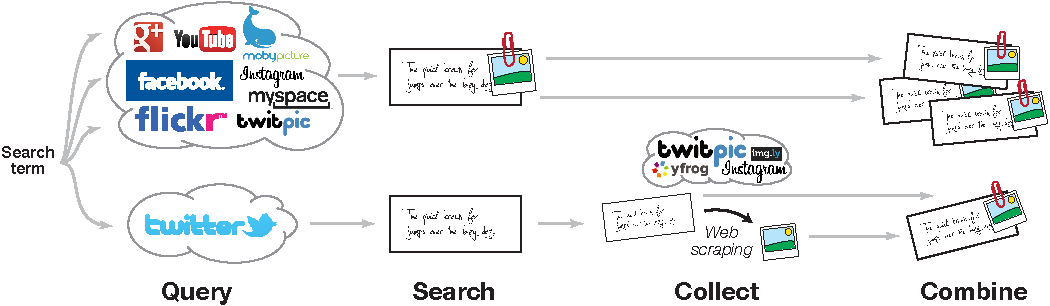
\includegraphics[width=0.8\linewidth]{./architecture.pdf}
\caption{Overview of the media collector: hybrid approach for the media item extraction process using a~combination of API access and Web scraping}
\label{fig:architecture}
\end{figure*}

\begin{lstlisting}[language=JavaScript,caption={Sample output of the media collector showing a~\mbox{Google+} post (edited for legibility, URLs shortened).},label={lst:media}]
{
  "mediaurl": "http://t.co/ubagkiR9",
  "storyurl": "https://t.co/dau5pBWD",
  "message": {
    "text": "My wife, who once said her vision of
        heaven was being on the lawn bouncing
        around beach balls at a Beach Boys
        concert [...]
        <a href=\"http://t.co/pH2OV1fW\" >
        http://t.co/pH2OV1fW</a> [...]",
    "clean": "My wife, who once said her vision of
        heaven was being on the lawn bouncing
        around beach balls at a Beach Boys
        concert [...]"
  },
  "user": "https://t.co/gIf2UVZR",
  "type": "photo",
  "timestamp": 1329342797000,
  "published": "2012-02-15T21:53:17.000Z"
}
\end{lstlisting}

\subsection{Magazine Layout}
In order to create the illusion of a~real magazine,
flipping from page to page needs to be as credible as possible.
The open-source library turn.js by Emmanuel García~\cite{TurnJs2012}
allows for the dynamic creation of magazines solely based on HTML5 technologies
with a~very realistic page flip effect.
We treat each event as one page of the magazine,
add the event metadata as headline and subheading of the page,
and arrange the images and accompanying microposts to fill the page.
For each event, we use the image with the highest resolution
as background image of the page in order to create a~lifestyle magazine appearance.

\subsection{Installation Instructions}
The NiteOutMag\texttrademark application requires the Chrome browser.
Download the application from the URL \todo{Add demo link} to the local file system.
Once there, drag and drop it into the \url{chrome://chrome/extensions/} page in the browser.
When you drop it on the extensions page, you will notice an install option popping up there.
When you agree to install, you will see the standard installation dialog
that informs you about the rights that the application is requesting.
It needs access to the before-mentioned event databases and media search APIs.

\section{Experiments}

\subsection{Query Examples}

\subsection{Discussion}

\section{Future Work and Conclusion}

% \section{Acknowledgments}
% Double-blind review process, need to remove for now


\bibliographystyle{abbrv}
\bibliography{acm2012grandchallenge}

\balancecolumns
\end{document}
